\chapter{Background}\label{chap:background}

\section{RocksDB}
RocksDB is an embedded key-value store optimized for modern flash storage.
RocksDB started out at Facebook, with the goal of making a version of Google's
LevelDB that performed well on modern hardware. Today, RocksDB is used at the
heart of a wide variety of databases, such as CockroachDB~\cite{cockroach},
MyRocks~\cite{myrocks} (Facebook's fork of MySQL) and TiDB~\cite{tidb}.

Traditional B-tree based database systems are often faced with poor write
performance as a result of random writes, which perform worse than sequential
writes on both magnetic and flash based storage mediums. RocksDB, on the other
hand, achieves impressive write performance through the use of immutable
log-structured merge trees~\cite{lsm} (LSM-trees), avoiding the need for random
writes to persistent storage altogether.

Writes are initially only written to a persistent write-ahead log (WAL) and
in-memory data structures referred to as memtables. Later these memtables are
flushed to their equivalent data structures on disk, Static Sorted Tables (SST).
The latter is done by background threads, allowing regular processing to
continue without getting backed by slow writes to persistent storage. Both of
these components originate in Patrick O'Neil's original paper on LSM-trees,
where the in-memory data structure is referred to as $ C_0 $, and the on-disk
structures $ C_{1..n} $.

% TODO:
% * Calling into RocksDB (C-API, rust-rocksdb)
% * Iterators
% * Prefix Iteration/Slice Transform

\subsection{MemTables}
All writes are initially synchronously written to an in-memory data structure---a
memtable---which is later flushed to disk at the point of filling up. Both the
size and the number of memtables can be configured at runtime.

RocksDB's default memtable implementation is a skiplist, with an $ O(\log n) $
bound on inserts, searches and deletes. This can be changed to a series of hash
based implementations, which offer better performance if all operations are done
within a pre-specified key prefix.

\subsection{Static Sorted Tables}
After a memtable reaches a certain size, RocksDB's background threads takes over
and flushes it to persistent storage. This will generate one or more SS-tables
on disk, where each file is sorted. SS-tables are immutable: a new SS-table is
always created, and existing ones are never updated. This ensures that writes
remain sequential.

\subsection{Write-Ahead Log}
RocksDB achieves durability through the use of a write-ahead log (WAL). Without
it, data in memtables would be lost at the event of a crash. By default, every
\code{Put} operation results in a write to the RocksDB WAL, with the optional
possibility of waiting for the write to be fully synchronized to the WAL before
returning.

Each memtable corresponds to a WAL-file, which is marked as obsolete obsolete
when the memtable has been safely persisted to disk. Each WAL-file includes a
sequence number, and the files are iterated through in order during recovery.
The WAL itself is built up of a sequence of records, where each record includes
a cyclic redundancy check (CRC) computed hash over the payload to maintain
integrity~\cite{rocksdb-wal}.

Optionally, the WAL can be written to a different directory than the regular
database files. This is essential for production systems that want to maintain a
high write throughput: compactions and memtable flushes can then utilize the
full disk capacity without slowing down the throughput of WAL writes. Even more
drastically, the database files could be written to faster, volatile storage,
relying solely on never-archived WAL-files for (albeit much slower) recovery.

\begin{listing}[H]\label{lst:write-batch}
  \begin{minted}[frame=lines]{rust}
let batch = WriteBatch::default()
batch.put("a", "1");
batch.put("b", "2");

let opts = WriteOptions::default();
opts.set_sync(true);
db.write(batch, &opts);
  \end{minted}

  \caption{Rust code for safely persisting a batch of writes to RocksDB and its
  write-ahead log.}
\end{listing}

\code{Put} operations can also be batched into a \code{WriteBatch} (as shown in
listing~\ref{lst:write-batch}), to amortize the cost of synchronizing the WAL
over a larger amount of write operations. This is an atomic operation: either
all the writes in the write batch succeeds, or none do.

\subsection{Basic Operations}
Akin to other key-value databases, RocksDB offers a familiar API of
\code{Put(key, value)}, \code{Get(key)} and \code{Delete(key)}, operating
directly on bytestream values. Both insertions and deletions are purely
sequential: subsequent \code{Put} operations of the same key never backtrack and
overwrite existing keys, and deletions insert tombstone markers to avoid having
to randomly read and mutate previously written values.

Whereas both memtables and SS-tables are sorted, each tree structure might
overlap with another. This is a result of the immutability property, and newly
created SS-tables might contain key ranges already included in existing
structures. This means that read operations in RocksDB, and other LSM-tree based
storage systems, have to iterate through each tree structure---starting with the
memtables---in an attempt to find the key in question. Reads within each sorted
tree structure can be done in $ O(\log n) $ through a binary search.

Going through a potentially large amount of SS-tables on disk is costly however,
and RocksDB employs a series of tricks to avoid doing so.

\subsection{Compactions}
To maintain immutability, new SS-tables are always created without modifying
existing on-disk content. Two writes to the same key can thus co-exist in
different SS-tables, even if only the last written key is relevant to the
system. This is quite wasteful, and would overtime lead to worse and worse read
performance. \cite{lsm} solves this through \textit{merging} existing LSM-trees
into new ones at regular intervals. RocksDB does so in background threads, where
it is referred to as \textit{compaction}.

During compacting, multiple SS-tables are merge-sorted into a single new
structure. This process also removes duplicate keys, retaining only the last
value for future use. Tombstones are also filtered out, together with any values
they might have deleted.

\begin{figure}[H]
  \centering
  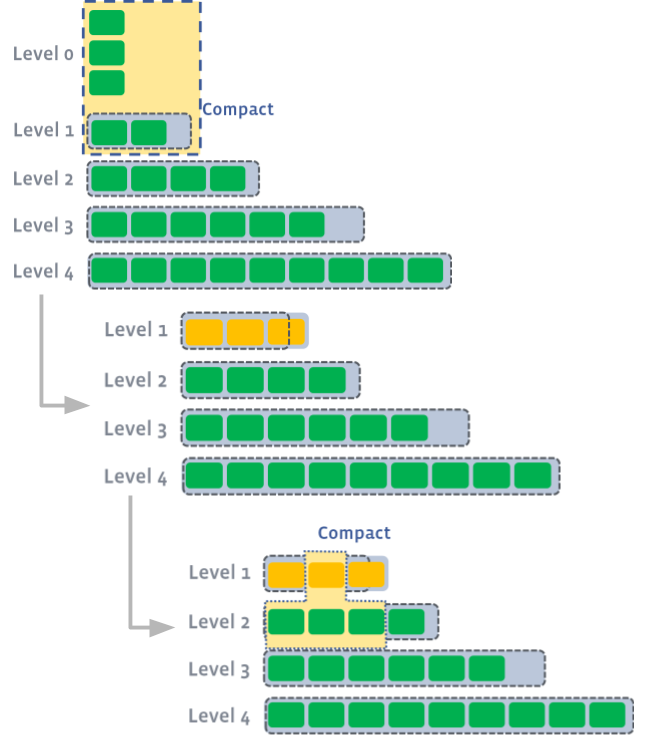
\includegraphics[width=0.5\textwidth]{level_compaction}
  \caption{SS-tables from initial levels are compacted into the next~\cite{rocksdb-compaction}.}
\end{figure}

In RocksDB, compactions are triggered when the previous \textit{level} reaches a
certain size. Referred to as \textit{leveled compaction}, this was one of the
original contributions of LevelDB\@. As described in~\cite{rocksdb-compaction},
this is usually initiated when the amount of SS-tables at the first level, level
0, goes beyond a certain amount. This in turn might cause the next level to go
beyond its size limit, resulting in a compaction to the next level again, and so
on. Unlike LevelDB, RocksDB also supports doing compactions in parallel, as long
as there are enough available background threads to do so.

\subsection{Bloom filters}
Iterating through every SS-table available to find a single key is inefficient.
Instead, we would like to ask the question ``can this key possibly exist here?''
for each of the SS-tables we go through, and only operate on the ones where the
answer is ``yes''. With a regular hash based data structure this would be quite
costly in terms of space, as we would need to maintain such a structure for
every SS-table in our database. Instead, RocksDB, and many other systems like
it, rely on a probabilistic data structure known as a bloom filter~\cite{bloom}
to do so.

Instead of knowing with 100\% certainty whether a key exists in a set, a bloom
filter would let us know if that key \textit{might possibly} be in the set, or
if it is \textit{definitely} not. The third option, of possibly \textit{not}
being in the set is impossible. The positive trade-off here is that it uses
significantly less space, opening the possibility of using it for every SS-table
in the system.

\subsection{Iteration}
One of the essential features of RocksDB compared to other key-value stores is
that its data is \textit{sorted}, and that it can be queried as such through
\textit{iterators}. This opens for a wide variety of possibilities that would
not have been feasible with a regular key-value store, such as range queries.
RocksDB supports iterating both forwards and backwards.

Similar to with reads, performing a fully ordered scan in an LSM-tree based
storage engine is far from optimal: every tree-structure, or SS-table in
RocksDB, needs to be considered, and as key ranges may overlap between different
files, sorted.

A lot of applications do not rely on completely random scans of keys however,
and only need support for ordered queries within a specific \textit{key prefix}.
Developers instruct RocksDB on how to retrieve a specific prefix from each key,
which RocksDB then internally uses to organize the data in such a manner that
iterating through keys within a \textit{specific prefix} is efficient: either by
storing bloom filters for each prefix, or by managing a hash based index
structure based on the prefix.

% TODO: might show an example to better explain prefix stuff here, or save it
% for implementation.
